\documentclass{amsart}
\usepackage{fullpage}

\usepackage[T1]{fontenc}
\usepackage[utf8]{inputenc} 
\usepackage{lmodern}
%\usepackage{concrete}
\usepackage[slovene]{babel}
\usepackage{amsmath,amssymb,amsfonts}
\usepackage{bbm}

\usepackage{tikz}
\usepackage{pgfplots}
\usepgfplotslibrary{fillbetween}
\usetikzlibrary{intersections}
\pgfplotsset{compat=newest}

\linespread{1}

\newcommand{\N}{\mathbb{N}}
\newcommand{\Z}{\mathbb{Z}}
\newcommand{\Q}{\mathbb{Q}}
\newcommand{\R}{\mathbb{R}}
\newcommand{\C}{\mathbb{C}}

% ukazi za matematicna okolja
\theoremstyle{definition} % tekst napisan pokoncno
\newtheorem{definicija}{Definicija}[section]
\newtheorem{primer}[definicija]{Primer}
\newtheorem{opomba}[definicija]{Opomba}

\renewcommand\endprimer{\hfill$\diamondsuit$}


\theoremstyle{plain} % tekst napisan posevno
\newtheorem{lema}[definicija]{Lema}
\newtheorem{izrek}[definicija]{Izrek}
\newtheorem{trditev}[definicija]{Trditev}
\newtheorem{posledica}[definicija]{Posledica}

\title{Seminarska naloga}
\author{Janez Podlogar}
\date{\today}

\begin{document}

\maketitle
\section{Navodilo naloge}
Streljamo v tarčo kvadratne oblike z robom $a$. Predpostavimo, da vsak zadetek zadene
tarčo in da je točka zadetka porazdeljena enakomerno po tarči. Izračunaj verjetnost, da
bo naš strel zadel bližje središču tarče kot njenemu robu.

\section{Definicje, trditve in izreki}

Spodaj so definicje in trditve, ki smo jih spoznali pri Analizi 3, na katere se bomo sklicali tekom naloge.

\begin{definicija}\label{def}
Množica $ A \subseteq \R^n $ ima \emph{mero $0$}, če za za vsak $\varepsilon > 0$ obstaja največ števno mnogo
kvadratov $k_1,K_2,K_3,\ldots$, da velja
\begin{equation*}
    A \subseteq K_1 \cup K_2 \cup K_3 \cup \ldots \text{ in } \sum_{j = 1}^{\infty} V(K_j) < \varepsilon
\end{equation*}
\end{definicija}

\begin{primer}\label{pri}
Pokažimo, da ima množica $A = \{ \R \times \{0\} \} \subseteq \R^2$ mero $0$.
Naj bo $ \varepsilon > 0 $ in $ K_j = \left[j,j+1\right] \times \left[0,\frac{\varepsilon}{2^{j+2}}\right] $ 
za $ k = 0,1,2,\ldots $ \\

Očitno velja prva zahteva:

\begin{equation*}
    A \subseteq \bigcup_{j=0}^{\infty} K_{j}
\end{equation*}

Z hitrim izračunom preverimo tudi drugo zahtevo

\begin{align*}
    \sum_{j = 0}^{\infty} V(K_j) 
    &= V(K_0) + V(K_1) + V(K_2) + \ldots \\
    &= \frac{\varepsilon}{4} + 2 * \sum_{j = 1}^{\infty} \frac{\varepsilon}{2^{j+2}} \\
    &= \frac{3*\varepsilon}{4} < \varepsilon
\end{align*}

Torej ima množica $A$ mero $0$.

\end{primer}

\begin{trditev}\label{trd}
    Naj bodo $B_1, B_2, B_3 \ldots $ množice z mero $0$. Tedaj ima $\bigcup_{j=1}^{\infty} B_{j}$ mero $0$.
\end{trditev}

% \begin{posledica}
%     Naj bo $f \colon \R^n \to \R $ zvezna. Potem ima njen graf mero $0$ v $\R^n$.
% \end{posledica}

\begin{izrek}[Lebesgueov izrek]\label{izr}
    Naj bo $f \colon K \to \R $ omejena, potem je $f$ integrabilna na $K$ natanko tedaj, ko ima množica
    v katerih $f$ ni zvezna mero $0$.
\end{izrek}

\section{Reštev}

Naj bo $T_a = \left[ -\frac{a}{2} , \frac{a}{2}\right]\times\left[-\frac{a}{2},\frac{a}{2}\right]$
tarča. Ker so zadetki porazdeljeni enakomerno, ima gostoto

\begin{equation*}
    f(x,y) = 
    \begin{cases}
        \frac{1}{a^2} & \text{če $ (x,y) \in T_a  $} \\
        0 & \text{sicer}
    \end{cases}
\end{equation*}

Gostota $f(x,y)$ zvezna skoraj povsod, saj ima posledično po primeru \eqref{pri} in trditvi 
\eqref{trd} množica točk nezveznosti mero $0$.

\begin{figure}[h]
    \centering
    \begin{tikzpicture}[scale=0.8]
        \begin{axis}[
            axis equal image,
            axis lines=center,
            xlabel={$x$}, xmin=-1.5, xmax=1.5,
            ylabel={$y$}, ymin=-1.5, ymax=1.5,
            ]
            \draw[red, thick, dotted] (-1,-1) rectangle (1,1);
        \end{axis}
    \end{tikzpicture}
    \caption{Točke nezveznosti pri $a=1$}
\end{figure}

Ker je $f$ na $\R^2$ omejena, je po Lebesgueovem izreku \eqref{izr} integrabilna na $\R^2$.
Sedaj lahko izračunamo verjetnost, da zadanemo znotraj nekega območja oziroma podmonožico 
$B \subseteq T_a$ tarče.

\begin{align*}
    P\big((x,y) \in B\big)
    &= \iint\limits_{\R^2} f(x,y) \, \mathbbm{1}_{B} \, \mathrm{d}x\mathrm{d}y \\
    &= \iint\limits_{B} f(x,y) \mathrm{d}x\mathrm{d}y
\end{align*}

Poiščimo množico točk, ki je bližje središču tarče kot kateremukoli izmed robov tarče.

\begin{figure}[!h]
    \centering
    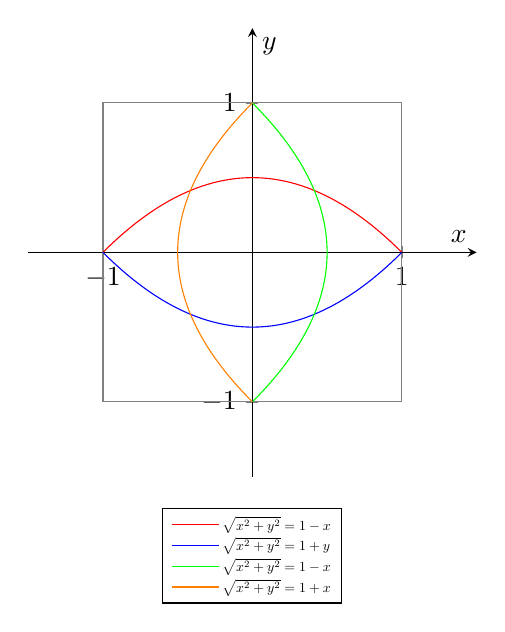
\begin{tikzpicture}[scale=1]
        \begin{axis}[
            axis equal image,
            %hide axis,
            axis lines=center,
            xlabel={$x$}, xmin=-1.5, xmax=1.5,
            ylabel={$y$}, ymin=-1.5, ymax=1.5,
            %extra x ticks={-1,1},
            %extra y ticks={-1,1},
            %extra tick style={grid=major},
            legend style={at={(0.5,-0.07)},anchor=north, legend cell align=left, nodes={scale=0.5, transform shape}},
            legend entries={$\sqrt{x^2+y^2}=1-x$, $\sqrt{x^2+y^2}=1+y$, $\sqrt{x^2+y^2}=1-x$, $\sqrt{x^2+y^2}=1+x$}
            ]
            \draw[gray, thin] (-1,-1) rectangle (1,1);
            \addplot[red, domain=-1:1, samples=100]({x},{((1-x^2)/2});
            \addplot[blue, domain=-1:1, samples=100]({x},{((x^2-1)/2});
            \addplot[green, domain=-1:1, samples=100]({(1-x^2)/2},{x});
            \addplot[orange ,domain=-1:1, samples=100]({(x^2-1)/2},{x});
        \end{axis}
    \end{tikzpicture}
    \caption{Roboni pogoji pri $a=1$}
\end{figure}

\begin{align}
    |(x,y)| < \frac{a}{2} - x \label{eq1} \\
    |(x,y)| < \frac{a}{2} - y \label{eq2} \\
    |(x,y)| < \frac{a}{2} + x \label{eq3} \\
    |(x,y)| < \frac{a}{2} + y \label{eq4}
\end{align}

Pogoj \eqref{eq1} opisuje vse točke, ki so bližje središču tarče kot desnemu robu tarče,
pogoj \eqref{eq2} opisuje vse točke, ki so bližje središču tarče kot spodnjemu robu tarče
pogoj \eqref{eq3} opisuje vse točke, ki so bližje središču tarče kot levemu robu tarče,
pogoj \eqref{eq4} opisuje vse točke, ki so bližje središču tarče kot zgornjemu robu tarče.
Točke, ki zadostijo vsem zgoraj napisanim enačbam so bližje središču kot robu, označimo jih z $S_a$.

Izračunati moramo
\begin{align*}
    P\big((x,y) \in S_a\big)
    &= \iint\limits_{S_a} f(x,y) \, \mathrm{d}x\mathrm{d}y \\
    &= \frac{1}{a^2}\iint\limits_{S_a} 1 \, \mathrm{d}x\mathrm{d}y
\end{align*}

Izračunati moramo ploščino pobarvanega območja.

    \begin{figure}[!h]
        \centering
        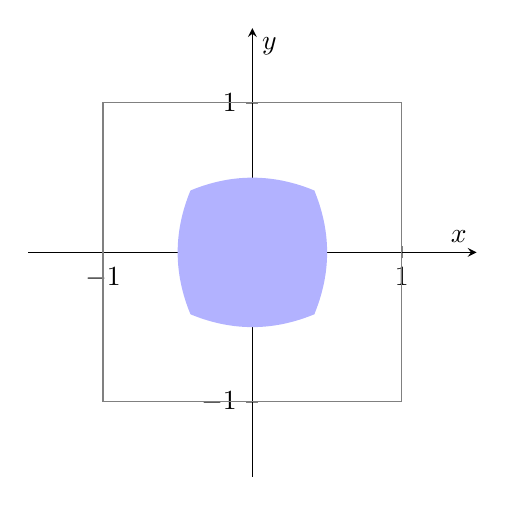
\begin{tikzpicture}[scale=1]
            \begin{axis}[
                axis equal image,
                %hide axis,
                axis lines=center,
                xlabel={$x$}, xmin=-1.5, xmax=1.5,
                ylabel={$y$}, ymin=-1.5, ymax=1.5,
                %extra x ticks={-1,1},
                %extra y ticks={-1,1},
                %extra tick style={grid=major},
                %legend style={at={(0.5,-0.07)},anchor=north, legend cell align=left, nodes={scale=0.5, transform shape}},
                %legend entries={$\sqrt{x^2+y^2}=1-x$, $\sqrt{x^2+y^2}=1+y$, $\sqrt{x^2+y^2}=1-x$, $\sqrt{x^2+y^2}=1+x$}
                ]
                \draw[gray, thin] (-1,-1) rectangle (1,1);
                \addplot[forget plot, draw=none, domain=-0.414:0.414, samples=100, name path=A]({x},{((1-x^2)/2});
                \addplot[forget plot, draw=none, domain=-0.414:0.414, samples=100, name path=B]({x},{((x^2-1)/2});
                \addplot[forget plot, draw=none, domain=-0.414:0.414, samples=100, name path=C]({(1-x^2)/2},{x});
                \addplot[forget plot, draw=none, domain=-0.414:0.414, samples=100, name path=D]({(x^2-1)/2},{x});
                \addplot[blue!30] fill between[of=A and B];
                \addplot[blue!30] fill between[of=C and D];
            \end{axis}
        \end{tikzpicture}
        \caption{Integral $\iint\limits_{S_1} 1 \, \mathrm{d}x\mathrm{d}y$}
    \end{figure}

\pagebreak

Ploščino najlažje izračunamo tako, da opazimo simetrijo rotacij in simetrijo zrcaljenja.
Izračunati ploščino območja le za enega izmed osmih trikotnikov.

\begin{figure}[!h]
    \centering
    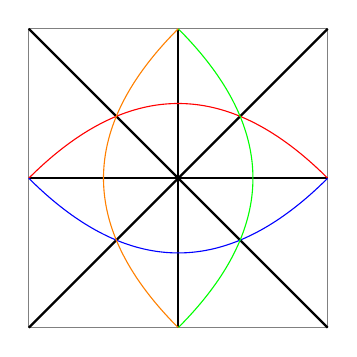
\begin{tikzpicture}[scale=1]
        \begin{axis}[
            axis equal image,
            hide axis,
            axis lines=center,
            xlabel={$x$}, xmin=-1.5, xmax=1.5,
            ylabel={$y$}, ymin=-1.5, ymax=1.5,
            %extra x ticks={-1,1},
            %extra y ticks={-1,1},
            %extra tick style={grid=major},
            legend style={at={(0.5,-0.07)},anchor=north, legend cell align=left, nodes={scale=0.5, transform shape}},
            %legend entries={$\sqrt{x^2+y^2}=1-x$, $\sqrt{x^2+y^2}=1+y$, $\sqrt{x^2+y^2}=1-x$, $\sqrt{x^2+y^2}=1+x$}
            ]
            \draw[gray, thin] (-1,-1) rectangle (1,1);
            \addplot[black, thick, domain=-1:1, samples=100]{x};
            \addplot[black, thick, domain=-1:1, samples=100]{-x};
            \addplot[black, thick, domain=-1:1, samples=100]{0};
            \addplot[black, thick, domain=-1:1, samples=100]({0},{x});
            \addplot[red, domain=-1:1, samples=100]({x},{((1-x^2)/2});
            \addplot[blue, domain=-1:1, samples=100]({x},{((x^2-1)/2});
            \addplot[green, domain=-1:1, samples=100]({(1-x^2)/2},{x});
            \addplot[orange ,domain=-1:1, samples=100]({(x^2-1)/2},{x});
        \end{axis}
    \end{tikzpicture}
    \caption{Simetrije}
\end{figure}

\begin{figure}[!h]
    \centering
    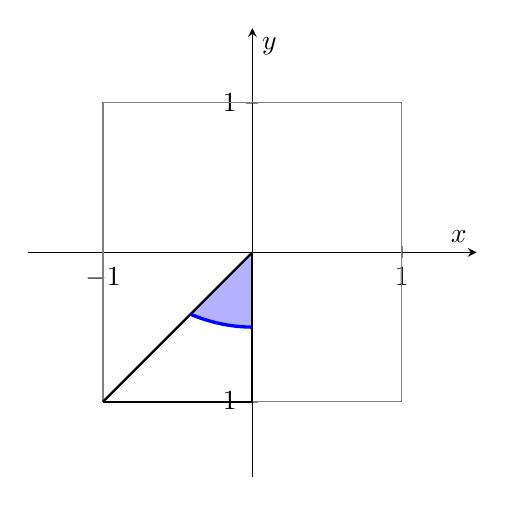
\begin{tikzpicture}[scale=1]
        \begin{axis}[
            axis equal image,
            %hide axis,
            axis lines=center,
            xlabel={$x$}, xmin=-1.5, xmax=1.5,
            ylabel={$y$}, ymin=-1.5, ymax=1.5,
            %extra x ticks={-1,1},
            %extra y ticks={-1,1},
            %extra tick style={grid=major},
            legend style={at={(0.5,-0.07)},anchor=north, legend cell align=left, nodes={scale=0.5, transform shape}},
            %legend entries={$\sqrt{x^2+y^2}=1-x$, $\sqrt{x^2+y^2}=1+y$, $\sqrt{x^2+y^2}=1-x$, $\sqrt{x^2+y^2}=1+x$}
            ]
            \draw[gray, thin] (-1,-1) rectangle (1,1);
            \addplot[black, thick, domain=-1:0, samples=100, name path=D]{x};
            \addplot[black, thick, domain=-1:0, samples=100]({0},{x});
            \addplot[black, thick, domain=-1:0, samples=100]({x},{-1});
            \addplot[blue, very thick, domain=-0.414:0, samples=100, name path=B]({x},{((x^2-1)/2});
            \addplot[blue!30] fill between[of=B and D];
        \end{axis}
    \end{tikzpicture}
    \caption{Osmina ploščine pri $a=1$}
\end{figure}

Funkcijo $|(x,y)| < \frac{a}{2} + y$, ki opisuje vse točke, ki so bližje središču tarče kot
spodnjemu robu tarče preoblikujemo v 
\begin{equation*}
    y = \frac{x^2}{a} - \frac{a}{4}
\end{equation*}
in poiščemo njeno presečišče z funkcijo $y = x$. Ko rešimo kvadratno enačbo,
dobimo za presečišče
\begin{equation*}
    x=\frac{a(1-\sqrt{2})}{2}
\end{equation*}
Sedaj lahko izračunamo ploščino območja. Najprej izračunamo območje pod pobarvanim delom.
\begin{align*}
    \Bigg| \int_{-\frac{a}{2}}^{0} \min \{ x, \tfrac{x^2}{a} - \tfrac{a}{4} \} \, \mathrm{d}x \Bigg|
    &= \Bigg| \int_{-\frac{a}{2}}^{\frac{a(1-\sqrt{2})}{2}} x \, \mathrm{d}x + \int_{\frac{a(1-\sqrt{2})}{2}}^{0} \tfrac{x^2}{a} - \tfrac{a}{4} \, \mathrm{d}x \Bigg|\\
    &= \frac{a^2}{3}(4\sqrt{2}-2)
\end{align*}
Da dobimo ploščino modrega območja, od ploščine trikotnika odštejemo dobljeni integral

\begin{align*}
    \frac{a^2}{8} - \frac{a^2}{24}(4\sqrt{2}-2)
    &= \frac{a^2}{8} (1 - \frac{1}{3}\big(4\sqrt{2}-2)\big) \\
    &= \frac{a^2}{8} ()
\end{align*}

\section{Simulacija}


\end{document} 